\documentclass[tikz=true]{standalone}
\usepackage{graphicx, standalone}
\usepackage[compat=1.1.0]{tikz-feynman}
\usepackage{tikz}
\usepackage{amsmath, amssymb}
\usepackage{euler}
\usepackage{fontspec}
\setmainfont{MinionPro}

\renewcommand{\k}{\ensuremath\text{k}}
\newcommand{\kp}{\ensuremath\text{k}'}
\newcommand{\q}{\ensuremath\text{q}}

\begin{document}

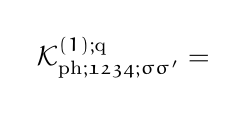
\begin{tikzpicture}[baseline=(current bounding box.center)]
	\node {$\mathcal{K}^{(1);\q}_{\text{ph};\mathfrak{1234};\sigma\sigma'}=$};
\end{tikzpicture}
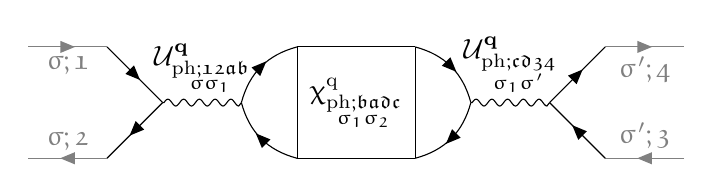
\begin{tikzpicture}[baseline=(current bounding box.center)]
	\begin{feynman}[small]
		\vertex (a1);
		\vertex[right=of a1] (b1);
		\vertex[below right=of b1] (c);
		\vertex[below left=of c] (b2);
		\vertex[left=of b2] (a2);
		\vertex[right=of c] (d);
		
		\vertex[above right=of d] (e1);
		\vertex[below right=of d] (e2);
		\vertex[right=1.5cm of e1] (f1);
		\vertex[right=1.5cm of e2] (f2);
		
		\vertex[below right=of f1] (g);
		\vertex[right=of g] (h);
		\vertex[above right=of h] (i1);
		\vertex[below right=of h] (i2);
		\vertex[right=of i1] (j1);
		\vertex[right=of i2] (j2);
		
		\node at ($(e1)!0.5!(f2)$) {$\chi^{\q}_{\substack{\text{ph};\mathfrak{badc}\\\sigma_1\sigma_2}}$};
		
		\diagram* {
			(a1) -- [gray, fermion, edge label'=$\sigma;\mathfrak{1}$] (b1) -- [fermion] (c) -- [fermion] (b2) -- [gray, fermion, edge label'=$\sigma;\mathfrak{2}$] (a2),
			(c) -- [photon, edge label=$\mathcal{U}^{\textbf{q}}_{\substack{\text{ph};\mathfrak{12ab}\\\sigma\sigma_1}}$] (d),
			(e2) -- [fermion, bend left=30] (d) -- [fermion, bend left=30] (e1),
			(e1) -- (f1) -- (f2) -- (e2) -- (e1),
			(f1) -- [fermion, bend left=30] (g) -- [fermion, bend left=30] (f2),
			(g) -- [photon, edge label=$\mathcal{U}^{\textbf{q}}_{\substack{\text{ph};\mathfrak{cd34}\\\sigma_1\sigma'}}$] (h),
			(j2) -- [gray, fermion, edge label'=$\sigma';\mathfrak{3}$] (i2) -- [fermion] (h) -- [fermion] (i1) -- [gray, fermion,edge label'=$\sigma';\mathfrak{4}$] (j1)
		};	
	\end{feynman}
\end{tikzpicture}

\end{document}